\documentclass{ximera}

\begin{document}
\title{Continuity and Discontinuity}
\begin{dialogue}
\item[Julia]What does it mean for a graph to be discontinuous? I don't get it!
\item[Dylan] I think it's like when there's a hole in the graph or something.
\item[James] Actually there are different kinds of discontinuities, but it's hard to visualize so let's take a look!
\item[Altogether] LET'S DIVE IN!
\end{dialogue}
\section{Introduction}
\begin{question}
A function $f$ is said to be \textit{continuous at a point} $x = a$ if which three conditions are satisfied?
\begin{selectAll}
\choice[correct]{$f(a)$ is defined}
\choice{$f(a) \neq 0$}
\choice[correct]{$\displaystyle \lim_{x\to a} f(x)$ exists}
\choice[correct]{$\displaystyle \lim_{x\to a} f(x)=f(a)$}
\choice{$f(x)$ is linear}
\choice{$f(x) \neq f(a)$}
\end{selectAll}
\end{question}
\subsection{Example}
Take the function $f(x) = \dfrac{(1-x)^2}{1-x}$.

\begin{image}
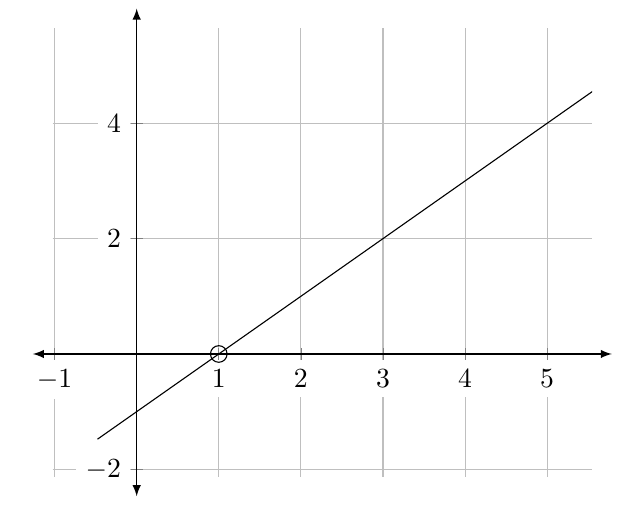
\begin{tikzpicture}
\begin{axis}[grid=both,
          xmax=5,ymax=5,
          axis lines=middle,
          restrict y to domain=-1.5:6.5,
          enlargelimits,
          axis line style={shorten >=-0.25cm,shorten <=-0.25cm,latex-latex},
          ticklabel style={fill=white}]
\addplot[domain=-5:7,mark=none,samples=200] {(x-1)} node[fill=white, below]{$y=\frac{(x-1)^2}{(x-1)}$};
\draw (axis cs:1,0) circle [radius=3pt];
\end{axis}
\end{tikzpicture}
\end{image}


Through some simple elimination, we can easily see that this function is equivalent to $1-x$, where $x \neq 1$. Thus, there is one point on the original function we should pay close attention to: $x=1$
\end{document}

%configuration={"latex_command":"latexmk -pdf -f -g -bibtex -synctex=1 -interaction=nonstopmode 'continuity.tex'"}